\[d_{\Delta t}(t) \leftrightarrow \frac{2\pi}{\Delta t}d_{\frac{2\pi}{\Delta t}}(\lambda)\]
\[f(t) \leftrightarrow F(\lambda)\]
\[f_{\Delta t}(t) = f(t)\cdot d_{\Delta t}(t) = \sum_{k = -\infty}^{+\infty} f(k\Delta t)\delta(t - k\Delta t) \leftrightarrow \frac{1}{2\pi}(F*\frac{2\pi}{\Delta t}d_{\frac{2\pi}{\Delta t}})(\lambda) =\]
\[= \frac{1}{\Delta t} \sum_{l = -\infty}^{+\infty} F(\lambda - \frac{2\pi l}{\Delta t}) = \frac{1}{\Delta t}F_{\frac{2\pi}{\Delta t}}^0(\lambda)|\cdot\Delta t H_{\frac{\Lambda}{2}}(\lambda)\]
Пусть $\exists \Lambda > 0 : F(\lambda) \equiv 0, \: |\lambda| > \frac{\Lambda}{2}$ --- ограниченый спектр, $\Rightarrow \frac{\pi}{\Delta t} \geq \frac{\Lambda}{2}$ не происходит наложение спектра.
$\Delta t = \frac{2\pi}{\Lambda}$ --- частота Найквиста.\\
\(F(\lambda) = F_{\frac{2\pi}{\Delta t}}^0(\lambda)\cdot H_{\frac{\Lambda}{2}}(\lambda)\), где $H_{\frac{\Lambda}{2}}(\lambda)$ --- оконная функция:
\begin{equation*}
H_{\frac{\Lambda}{2}}(\lambda) = 
 \begin{cases}
   1, |\lambda| \leq \frac{\Lambda}{2}\\
   0, \texttt{иначе}
 \end{cases}
\end{equation*}
\begin{equation*}
g(t) = 
 \begin{cases}
   1, |t| \leq \frac{\Lambda}{2}\\
   0, \texttt{иначе}
 \end{cases}
\end{equation*}
\[\leftrightarrow 2\frac{\sin(\lambda A)}{\lambda} = G(\lambda)\]
\[h_{\frac{\Lambda}{2}}(t) = \frac{1}{\pi}\frac{\sin(\frac{\Lambda}{2}t)}{t} \leftrightarrow H_{\frac{\Lambda}{2}}(\lambda)\]
\[\Delta t(f_{\Delta t} + h_{\frac{\Lambda}{2}}) \leftrightarrow f(\lambda)\]
Интероляционная формула Котельникова:
\[\Delta t \sum_{k = -\infty}^{+\infty} f(k\Delta t)\int_{-\infty}^{+\infty}\delta(t - s - k\Delta t)\cdot h_{\frac{\Lambda}{2}}(s)ds = \frac{\Delta t}{\pi} \sum_{k = -\infty}^{+\infty} f(k\Delta t)\frac{\frac{\Lambda}{2}\sin(t - k\Delta t)}{t - k\Delta t}\]
\begin{center}
        \includegraphics[width=1\textwidth, height = 0.37\textheight]{ch5/1.eps}
\end{center}
\begin{equation*}
h_{\frac{T}{2}}(t) = 
 \begin{cases}
   1, |t| \leq \frac{T}{2}\\
   0, \texttt{иначе}
 \end{cases}
\end{equation*}
\[H_{\frac{T}{2}}(\lambda) = \frac{2}{\lambda}\sin(\frac{T\lambda}{2})\]
Пример Ряби:
\begin{center}
        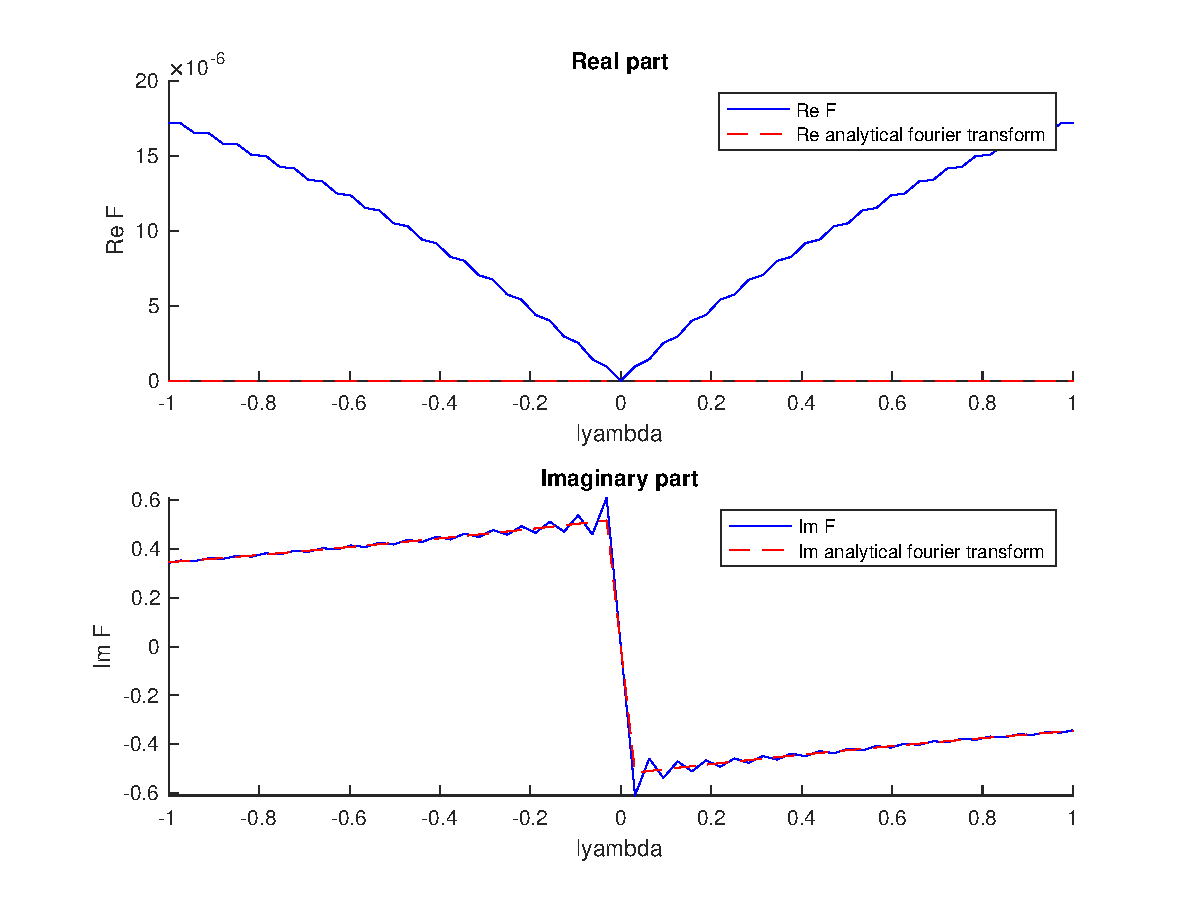
\includegraphics[width=1\textwidth]{ch5/pic_1_2.eps}
\end{center}
Введем функцию:
\begin{multline}
\widetilde{F} = F*d_{\frac{2\pi}{\Delta t}};\;\frac{T}{2\pi}(\widetilde{F}*sync(\frac{T}{2}\cdot))(\lambda) = \frac{T}{2\pi}\int_{-\infty}^{+\infty} \widetilde{F}(t - s)\frac{\sin(\frac{T}{2}s)}{\frac{T}{2}s}ds =\\
= \frac{T}{2\pi} \sum_{k = -\infty}^{+\infty} \int_{-\infty}^{+\infty} F(t - s - k\Delta t)\frac{\sin(\frac{T}{2})}{\frac{T}{2}s}ds
\end{multline}

Если $T$ достаточно большое: \[W_T(s) = \frac{T}{2\pi}\frac{\sin(\frac{T}{2}\lambda)}{\frac{T}{2}\lambda} \xrightarrow[T\to\infty] {\texttt{сл}} \delta(\lambda)\]
Теперь введем функцию $\widetilde{\widetilde{F}}:$
\[\widetilde{\widetilde{F}}(\lambda) = \frac{T}{2\pi}(\widetilde{F} + sync(\frac{T}{2}\cdot))(\lambda)\]

\newpage
Дискретизация $\widetilde{\widetilde{F}}$ 
\begin{center}
        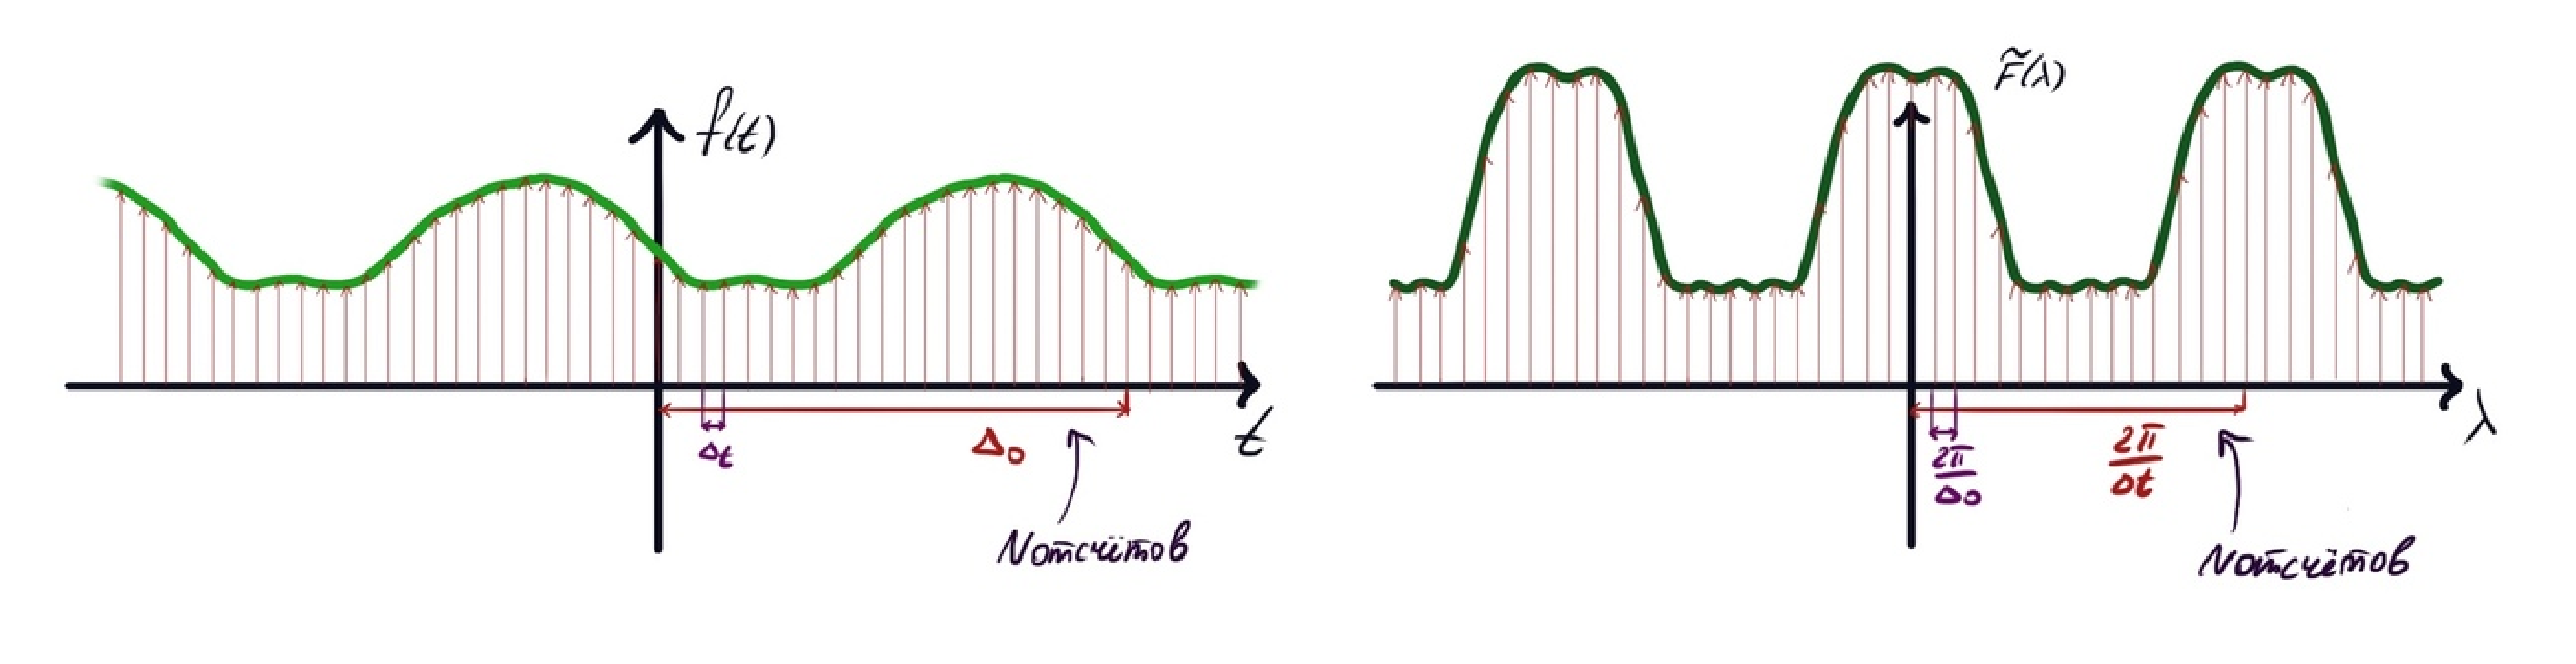
\includegraphics[width=1\textwidth]{ch5/2.eps}
\end{center}
\(\qquad \qquad \Big(f(\cdot)d_{\Delta t}(\cdot)h_{\frac{T}{2}}(\cdot)*d_{\Delta 0}\Big)(t)\qquad \qquad \qquad \qquad \frac{2\pi}{\Delta t\Delta 0}\widetilde{\widetilde{F}}(\lambda)\cdot d_{\frac{2\pi}{\Delta 0}}(\lambda)\)
\[\widetilde{f}_{\Delta t}(t) = \widetilde{f}(t)d_{\Delta t}(t) = \sum_{k = - \infty}^{+\infty} \widetilde{f}(k\Delta t)\delta(t - k\Delta t) \leftrightarrow \frac{1}{2\pi}\widetilde{F}*\frac{2\pi}{\Delta t}d_{\frac{2\pi}{\Delta t}} = \frac{1}{\Delta t}\widetilde{F}*d_{\frac{2\pi}{\Delta t}}\]
\begin{equation*}
\widetilde{h_{\Delta_0}}(t) = 
 \begin{cases}
   1, t \in [-\frac{\Delta t}{2}, \Delta_0 - \frac{\Delta t}{2}]\\
   0, \texttt{иначе}
 \end{cases}
\end{equation*}
\begin{equation*}
h_{\Delta_0}(t) = 
 \begin{cases}
   1, |t| \leq \frac{\Delta_0}{2}\\
   0, \texttt{иначе}
 \end{cases}
\end{equation*}
\[\widetilde{h_{\Delta_0}}(t) = h_{\Delta_0}(t - \frac{\Delta_0 + \Delta t}{2})\]
\[h_{\Delta_0}(t) \leftrightarrow \frac{2}{\lambda}\sin(\frac{\Delta_0 \lambda}{2})\]
\[\widetilde{H_{\Delta_0}}(\lambda) = e^{-\frac{i(\Delta_0 + \Delta t)\lambda}{2}}\]
\[\widetilde{f_{\Delta t}}(t)\widetilde{h_{\Delta_0}}(t) \leftrightarrow \frac{1}{\Delta t}\widetilde{F_{\frac{2\pi}{\Delta t}}^0}*\frac{1}{2\pi\lambda}\sin(\frac{\Delta_0\lambda}{2})\cdot e^{-\frac{i(\Delta_0 + \Delta t)\lambda}{2}} = \]
\[= \frac{1}{\Delta t}\int_{-\infty}^{+\infty} \sum_{l = -\infty}^{+\infty} \widetilde{F}(\lambda - \mu - \frac{2\pi l}{\Delta t})e^{-\frac{i(\Delta_0 + \Delta t)\mu}{2}}\frac{1}{2\pi\mu}\sin(\frac{\Delta_0 \mu}{2})d\mu\]
\[\widetilde{f}_{\Delta t}(t)\widetilde{h}_{\Delta_0}(t) = \sum_{k = 0}^{N - 1} \widetilde{f}(k\Delta t)\delta(t - k\Delta t)\]
\[\widetilde{\widetilde{f}}(t) = ((\widetilde{f}_{\Delta t}\cdot \widetilde{h}_{\Delta_0})*d_{\Delta_0})(t) = \sum_{m = -\infty}^{+\infty} \widetilde{f}(k\Delta t)\delta(t - k\Delta t - m\Delta_0)\]
\[\frac{1}{\Delta t}\frac{2\pi}{\Delta_0}\widetilde{\widetilde{F}}d_{\frac{2\pi}{\Delta_0}}(\lambda) = \sum_{n = -\infty}^{+\infty} \alpha_n\delta(\lambda - \frac{2\pi}{\Delta_0}n)\]
\[\widetilde{f}(t_k) : \widetilde{f}_0, ..., \widetilde{f}_{N - 1} \rightarrow \alpha_0, ..., \alpha_{N - 1} --- ?\]
Найдем формулу:
\[\widetilde{\widetilde{f}}(t) = \frac{1}{2\pi}\int_{-\infty}^{+\infty}(\sum_{n = -\infty}^{+\infty} \alpha_n\delta(\lambda - \frac{2\pi n}{\Delta_0}))e^{i\lambda t}d\lambda = \frac{1}{2\pi}\sum_{n = -\infty}^{+\infty} \alpha_n e^{\frac{2\pi int}{\Delta_0}}\]
\[\frac{1}{2\pi}\alpha_n = \frac{1}{\Delta_0}\int_{-\frac{\Delta t}{2}}^{\Delta_0 - \frac{\Delta t}{2}} \widetilde{\widetilde{f}}(t)e^{-i\lambda t}dt\]
\[\alpha_n = \frac{2\pi}{\Delta_0}\int_{-\frac{\Delta t}{2}}^{\Delta_0 - \frac{\Delta t}{2}} \sum_{n = -\infty}^{+\infty} \sum_{k = 0}^{N - 1} \widetilde{f}(k\Delta t)\delta(t - k\Delta t - m\Delta_0)e^{-\frac{2\pi int}{\Delta 0}}dt\]
Ненулевое только при $m = 0$
\[m \geq 1 ;\;\; t - k\Delta t - m\Delta_0 \leq \Delta_0 - \frac{\Delta t}{2} - \Delta_0 < 0\]
\[m \leq -1 ;\;\; t - k\Delta t - m\Delta_0 \geq -\frac{\Delta t}{2} - N\Delta t + \Delta t + \Delta_0 \geq \frac{\Delta t}{2} > 0 \Rightarrow\]
При $m \neq 0$ нулевые слагаемые.
\[\alpha_n = \frac{2\pi}{\Delta_0}\int_{-\frac{\Delta t}{2}}^{\Delta_0 - \frac{\Delta t}{2}} \sum_{k = 0}^{N - 1} \widetilde{f}(k\Delta t)\delta(t - k\Delta t - m\Delta_0)e^{-i\lambda t}dt = \frac{2\pi}{\Delta_0}\sum_{k = 0}^{N - 1} \widetilde{f}(k\Delta t)e^{-\frac{2\pi ink}{N}} \]
\(\{\frac{\Delta t}{\Delta_0} = \frac{1}{N}\}\)
\[\alpha_n \approx \frac{2\pi}{\Delta_0\Delta t}\widetilde{F}(\lambda_n);\;\;\lambda_n = \frac{2\pi n}{\Delta_0},\; n = 0, ..., N - 1\]
\[\widetilde{F}(\lambda_n) = \widetilde{F}_n \approx \Delta t\sum_{k = 0}^{N - 1}\widetilde{f}_ke^{\frac{2\pi ink}{N}}\]
ПДПФ: \[F_n = \sum_{k = 0}^{N - 1} f_k e^{-\frac{2\pi ink}{N}},\; n = 0, ..., N - 1\]
ОДПФ: \[f_k = \sum_{n = 0}^{N - 1} F_n e^{\frac{2\pi ink}{N}},\; k = 0, ..., N - 1\]
\[\widetilde{F}(\lambda_n) = \widetilde{F}_n,\; n = 0, ..., [\frac{N}{2}];\;\widetilde{F}(-\frac{2\pi}{\Delta_0}) = \widetilde{F}_{N - 1};\; \widetilde{F}(\frac{2\pi n}{\Delta_0}) \approx \widetilde{F}_n(\mod N)\]
\[F(\lambda) = \int_{-\infty}^{+\infty} f(t)e^{-i\lambda t}dt \approx \sum_{k = -\infty}^{+\infty} f(k\Delta_t)e^{-i\lambda k\Delta t}\Delta t\]
\[\lambda = \frac{2\pi n}{\Delta_0};\;\; F(\frac{2\pi n}{\Delta_0}) \approx \Delta t\sum_{k = -\infty}^{+\infty} f(k\Delta t)e^{-\frac{2\pi ink\Delta t}{\Delta_0}} = \Delta t\sum_{k = 0}^{N - 1} f(k\Delta t)e^{-\frac{2\pi ink}{N}}\]
\section{Оценка погрешности}
\subsection{Эффект наложения спектров}
Пусть: 
\begin{multline}
f \in C^2(-\infty, +\infty)\\
\int_{-\infty}^{+\infty} |f(t)|dt < \infty;\;\int_{-\infty}^{+\infty} |f^{'}(t)|dt < \infty;\;\int_{-\infty}^{+\infty} |f^{''}(t)|dt \leq c < \infty
\end{multline}
\[f^{''}(t) \leftrightarrow (i\lambda)^2F(\lambda) = \int_{-\infty}^{+\infty} f^{''}(t)e^{-i\lambda t}dt;\;\;\lambda^2|F(\lambda)| \leq c;\;\; \lambda \neq 0;\;\; |F(\lambda)| \leq \frac{c}{\lambda^2}\]
\[f_{\Delta t}(t) \leftrightarrow \frac{1}{\Delta t}\sum_{l = -\infty}^{+\infty} F(\lambda - \frac{2\pi l}{\Delta t}) = \frac{1}{\Delta t}(F(\lambda) + \sum_{l \neq 0} F(\lambda - \frac{2\pi l}{\Delta t}))\]
\[\sum_{l \neq 0} F(\lambda - \frac{2\pi l}{\Delta t})) \texttt{ --- ошибка наложения спектра.}\]
\[|\sum_{l \neq 0} F(\lambda - \frac{2\pi l}{\Delta t}))| \leq \sum_{l \neq 0} \frac{c}{(\lambda - \frac{2\pi l}{\Delta t})^2} \leq \{(*)\} \leq \frac{2c(\Delta t)^2}{\pi^2} \sum_{l = 1}^{+\infty} \frac{1}{(2l - 1)^2} < \varepsilon\]
\[(*) \; l > 0;\; |\lambda - \frac{2\pi l}{\Delta t}| \geq \frac{2\pi l}{\Delta t} - |\lambda| \geq \frac{2\pi l}{\Delta t} - \frac{\Lambda}{2} > \{\frac{\Lambda}{2} < \frac{\pi}{\Delta t}\} > \frac{\pi}{\Delta t}(2l - 1)\]
\subsection{Рябь($\Delta_0 > 0$)}
\begin{equation*}
h_{\Delta_0}(t) = 
 \begin{cases}
   1, |t| \leq \frac{\Delta_0}{2}\\
   0, \texttt{иначе}
 \end{cases}
\end{equation*}
\[f(t)\cdot h_{\Delta_0}(t) \leftrightarrow \frac{1}{2\pi}F*H_{\Delta_0}(\lambda) = \{H_{\Delta_0}(\lambda) = \frac{2}{\lambda}\sin(\frac{\Delta_0\lambda}{2})\} = (F*\frac{1}{\pi\lambda}\sin(\frac{\Delta_0\cdot}{2}))(\lambda) = \]
\(= \int_{-\infty}^{+\infty} F(\lambda - \mu)\frac{\sin(\frac{\Delta_0\mu}{2})}{\pi\mu}d\mu\)
\[F(\lambda) = F(\lambda)\int_{-\infty}^{+\infty} \frac{\sin(\frac{\Delta_0\mu}{2})}{\pi\mu}d\mu\]
\[h_{\Delta_0}(t) = \frac{1}{2\pi}\int_{-\infty}^{+\infty} \frac{2}{\mu}\sin(\frac{\Delta_0\mu}{2})e^{-i\mu t}d\mu\]
\subsection{Ошибка ряби}
\[I = \int_{-\infty}^{+\infty} [F(\lambda - \mu) - F(\lambda)]\frac{\sin(\frac{\Delta_0\mu}{2})}{\pi\mu}d\mu\]
\begin{enumerate} 
   \item $F$ непрерывна при $\lambda = \lambda_0$
   \item Пусть $F(\lambda_0 \pm 0) ;\; F(\lambda_0 - 0) \neq F(\lambda_0 + 0)$
\end{enumerate}
\[I = \int_{-\infty}^{+\infty} [F(\lambda - \mu) - F(\lambda)]\frac{\sin(\frac{\Delta_0\mu}{2})}{\pi\mu}d\mu\]
a). $F$ непрерывна по $\lambda;\; \Lambda > 0;\; |\lambda| \leq \frac{\Lambda}{2}$
\begin{equation*}
f(\cdot) :
 \begin{cases}
   \int_{-\infty}^{+\infty} |f(t)|dt \leq c_0 < +\infty\\
   \int_{-\infty}^{+\infty} |tf(t)|dt \leq c_1 < \infty\\
   \int_{-\infty}^{+\infty} |tf^{'}(t)|dt \leq \widetilde{c_1} < \infty
 \end{cases}
\end{equation*}
$\varepsilon > 0$ Задача: найти ограничение на $\Delta_0:$
\[|I| \leq \varepsilon;\; \delta = \frac{\varepsilon\pi}{6c_1} > 0\]
\begin{multline}
I = \int_{-\delta}^{\delta} [F(\lambda - \mu) - F(\lambda)]\frac{\sin(\frac{\Delta_0\mu}{2})}{\pi\mu}d\mu + \int_{|\mu| \geq \delta} F(\lambda - \mu)\frac{\sin(\frac{\Delta_0\mu}{2})}{\pi\mu}d\mu - \\
- \int_{|\mu| \geq \delta}F(\lambda)\frac{\sin(\frac{\Delta_0\mu}{2})}{\pi\mu}d\mu
\end{multline}
\[1). |I_1| \leq \int_{-\delta}^{\delta} |F(\lambda - \mu) - F(\lambda)|\frac{|\sin(\frac{\Delta_0\mu}{2})|}{|\pi\mu|}d\mu \leq \frac{c_1}{\pi} \int_{-\delta}^{\delta} |\sin(\frac{\Delta_0\mu}{2})| \leq \frac{2\delta c_1}{\pi} = \frac{\varepsilon}{3}\]
\[\{ F(\lambda) = \int_{-\infty}^{+\infty} f(t)e^{-i\lambda t}dt;\;F^{'}(\lambda) = \int_{-\infty}^{+\infty} (-it)f(t)e^{-i\lambda t}dt\}\]
\[\Rightarrow F^{'}(\lambda) \leq c_1 \Rightarrow |F(\lambda - \mu) - F(\lambda)| \leq c_1|\mu|\}\]
\[|\mu| \geq \delta;\; |\frac{F(\lambda - \mu)}{\pi\mu}| \leq \frac{c_0}{\pi\delta} = \alpha_0\]
\[(-it)f(t) = \frac{1}{2\pi}\int_{-\infty}^{+\infty} F^{'}(\lambda)e^{i\lambda t}d\lambda| \cdot \frac{d}{dt}\]
\[-i(f(t) + tf^{'}(t)) = \frac{1}{2\pi}\int_{-\infty}^{+\infty} F^{'}(\lambda)(i\lambda)e^{i\lambda t}d\lambda\]
\[(i\lambda)F^{'}(\lambda) = i\int_{-\infty}^{+\infty} [f(t) + tf^{'}(t)]e^{-i\lambda t}dt\]
\[|\lambda||F^{'}(\lambda)| \leq c_0 + \widetilde{c}_1; \; |\frac{F(\lambda - \mu)}{\mu\pi}| \leq \alpha_0\]
\[|\frac{F^{'}(\lambda - \mu)}{\mu\pi}| \leq \frac{c_0 + \widetilde{c}_1}{\pi|\mu||\lambda - \mu|} = \frac{c_0 + \widetilde{c}_1}{\pi|\mu|(|\mu| - |\lambda|)} \leq {(**)} \leq \frac{c_0 + \widetilde{c}_1}{\pi(\mu^2 - |\mu|\frac{\Lambda}{2})} \leq \frac{2(c_0 + \widetilde{c}_1)}{\pi\mu^2}\]
\[(**) \; |\mu| - \frac{\Lambda}{2} \leq |\mu| - |\lambda| \leq (\mu - \lambda);\]
\[\mu| \geq \max(\delta, \Lambda);\; \frac{\mu^2}{2} \leq \mu^2 - |\mu|\frac{\Lambda}{2} \leftrightarrow \frac{\mu^2}{2} - |\mu|\frac{\Lambda}{2} = |\mu|(|\mu| - \Lambda) > 0\]
\[|\frac{d}{d\mu}[\frac{F(\lambda - \mu)}{\pi\mu}]| = \frac{1}{\pi}|-\frac{F^{'}(\lambda - \mu)\mu - F(\lambda - \mu)}{\mu^2}| = \frac{1}{\pi}[\frac{F^{'}(\lambda - \mu)}{\mu} + \frac{F(\lambda - \mu)}{\mu^2}] \leq\]
\(\leq \frac{2(c_0 + \widetilde{c}_1)}{\pi\mu^2} + \frac{c_0}{\pi\mu^2} = \frac{3c_0 + 2\widetilde{c}_1}{\pi}\frac{1}{\mu^2} = \frac{\widetilde{\alpha}_1}{\mu^2}\)
\(2).R > 0;\; R > \Lambda > 0\)
\[I_2^R = \int_{R \geq |\mu| \geq \delta} F(\lambda - \mu)\frac{\sin(\frac{\Delta_0\mu}{2})}{\pi\mu}d\mu = -\frac{2}{\Delta_0}\int_{R \geq |\mu| \geq \delta} \frac{F(\lambda - \mu)}{\pi\mu}d(\cos(\frac{\Delta_0\mu}{2})) = \]
\[= \frac{2}{\Delta_0}\Big(-[\frac{F(\lambda - \mu)}{\pi\mu}\cos(\frac{\Delta_0\mu}{2})\bigg|_{\mu = -R}^{-\delta} + -||-\bigg|_{\mu = \delta}^R] + \int_{R \geq |\mu| \geq \delta} \frac{d}{d\mu}[\frac{F(\lambda - \mu)}{\pi\mu}]\cos(\frac{\Delta_0\mu}{2})d\mu\Big)\]
\[|I_2^R| \leq \frac{2}{\Delta_0}[4\alpha_0 + |\int_{R \geq |\mu| \geq \Lambda} \frac{d}{d\mu}[...]\cos(...)d\mu| + |\int_{\Lambda \geq |\mu| \geq \delta} \frac{d}{d\mu}[...]\cos(...)d\mu|] \leq \]
\(\leq \frac{2}{\Delta_0}[4\alpha_0 + \widetilde{\alpha}_1\int_{R \geq |\mu| \geq \Lambda} \frac{d\mu}{\mu^2} + |\int_{\Lambda \geq |\mu| \geq \delta} ...|]\)
\[\int_{-R}^{-\Lambda} \frac{d\mu}{\mu^2} = \frac{1}{\Lambda} - \frac{1}{R} \leq \frac{1}{\Lambda};\;\; \int_{\Lambda}^{R} \frac{d\mu}{\mu^2} = \frac{1}{\Lambda} - \frac{1}{R} \leq \frac{1}{\Lambda}\]
\[\Rightarrow |I_2^R| \leq \frac{2}{\Delta_0}[4\alpha_0 + \frac{2\widetilde{\alpha}_1}{\Lambda} + |\int_{\Lambda \geq |\mu| \geq \delta} ...d\mu|]\]
При $\Lambda \geq |\mu| \geq \delta:$
\[|\frac{d}{d\mu}[\frac{F(\lambda - \mu)}{\pi\mu}]| = \frac{1}{\pi}|\frac{F^{'}(\lambda - \mu)}{\mu} + \frac{F(\lambda - \mu)}{\mu^2}| \leq \frac{1}{\pi}[\frac{c_1}{\delta} + \frac{c_0}{\delta^2}] = \alpha_1\]
\[\Rightarrow |\int_{\Lambda \geq |\mu| \geq \delta} \frac{d}{d\mu}(...)cos(...)d\mu| \leq 2\Lambda\alpha_1 \Rightarrow |I_2^R| \leq \frac{2}{\Delta_0}[4\alpha_0 + \frac{2\widetilde{\alpha}_1}{\Lambda} + 2\Lambda\alpha_1]\]
\[R \rightarrow \infty \;\; |I_2| \leq \frac{1}{\Delta_0}[8\alpha_0 + \frac{4\widetilde{\alpha}_1}{\Lambda} + 4\Lambda\alpha_1] \leq \frac{\varepsilon}{3}\]
\[3). |I_3| \leq \frac{|F(\lambda)|}{\pi}|\int_{\mu \geq \delta} \frac{\sin(\frac{\Delta_0\mu}{2})}{\mu}d\mu| \leq \{\mu = \frac{2\psi}{\Delta_0};\;d\mu = \frac{2}{\Delta_0}d\psi\} \leq \frac{2c_0}{\pi}|\int_{\frac{\Delta_0\delta}{2}}^{+\infty} \frac{\sin(\psi)}{\psi}|d\psi\]
Пусть \(\frac{\Delta_0\delta}{2} = 2\pi k_0, \: k_0 \in \SetN;\; \Delta_0 = \frac{4\pi k_0}{\delta}\)
\[\int_{2\pi k_0}^{+\infty} \frac{\sin(\psi)}{\psi}d\psi = \sum_{l = k_0}^{+\infty} [\int_{2\pi l}^{\pi + 2\pi l} \frac{\sin(\psi)}{\psi}d\psi - \int_{\pi + 2\pi l}^{2\pi + 2\pi l} -\frac{\sin(\psi)}{\psi}d\psi] =\]
\(= \sum_{k = 2k_0}^{+\infty} (-1)^k\sigma_k\) -- ряд Лейбница.
\[0 < \sigma_{k + 1} \leq \sigma_k \leq \frac{1}{k};\; R_n = \sum_{k = n}^{+\infty} (-1)^k\sigma_k;\; \sigma_{2k_0} \geq \sigma_{2k + 1} \geq \sigma_{2k_0 + 2}\]
\[0 > R_{2k_0 - 1} = -\sigma_{2k_0 - 1} + R_{2k_0} \Rightarrow 0 \leq R_{2k_0} \leq \sigma_{2k_0 - 1} \leq \frac{1}{2k_0 - 1} \Rightarrow \frac{1}{2k_0 - 1} \leq \frac{\varepsilon\pi}{6c_0}\]
\[2k_0 - 1 \geq \frac{6c_0}{\varepsilon\pi} \Leftarrow k_0 \geq [\frac{3c_0}{\varepsilon\pi} + 1]\]
\[|I_3| \leq \frac{2c_0}{\pi}\int_{2\pi k_0}^{+\infty} \frac{\sin(\psi)}{\psi}d\psi \leq \frac{\varepsilon\pi 2c_0}{6c_0\pi} = \frac{\varepsilon}{3}\]
\begin{theorem}
Если $\Delta_0 \geq \max\{\frac{4\pi}{\delta}[\frac{3c_0}{\varepsilon\pi} + 1], \frac{3}{\varepsilon}[8\alpha_0 + 4\Lambda\alpha_1 + \frac{4\widetilde{\alpha}_1}{\Lambda}]\},$ то $|I| \leq \varepsilon.$
\end{theorem}